\documentclass{scrartcl}\usepackage[]{graphicx}\usepackage[]{color}
%% maxwidth is the original width if it is less than linewidth
%% otherwise use linewidth (to make sure the graphics do not exceed the margin)
\makeatletter
\def\maxwidth{ %
  \ifdim\Gin@nat@width>\linewidth
    \linewidth
  \else
    \Gin@nat@width
  \fi
}
\makeatother

\definecolor{fgcolor}{rgb}{0.345, 0.345, 0.345}
\newcommand{\hlnum}[1]{\textcolor[rgb]{0.686,0.059,0.569}{#1}}%
\newcommand{\hlstr}[1]{\textcolor[rgb]{0.192,0.494,0.8}{#1}}%
\newcommand{\hlcom}[1]{\textcolor[rgb]{0.678,0.584,0.686}{\textit{#1}}}%
\newcommand{\hlopt}[1]{\textcolor[rgb]{0,0,0}{#1}}%
\newcommand{\hlstd}[1]{\textcolor[rgb]{0.345,0.345,0.345}{#1}}%
\newcommand{\hlkwa}[1]{\textcolor[rgb]{0.161,0.373,0.58}{\textbf{#1}}}%
\newcommand{\hlkwb}[1]{\textcolor[rgb]{0.69,0.353,0.396}{#1}}%
\newcommand{\hlkwc}[1]{\textcolor[rgb]{0.333,0.667,0.333}{#1}}%
\newcommand{\hlkwd}[1]{\textcolor[rgb]{0.737,0.353,0.396}{\textbf{#1}}}%

\usepackage{framed}
\makeatletter
\newenvironment{kframe}{%
 \def\at@end@of@kframe{}%
 \ifinner\ifhmode%
  \def\at@end@of@kframe{\end{minipage}}%
  \begin{minipage}{\columnwidth}%
 \fi\fi%
 \def\FrameCommand##1{\hskip\@totalleftmargin \hskip-\fboxsep
 \colorbox{shadecolor}{##1}\hskip-\fboxsep
     % There is no \\@totalrightmargin, so:
     \hskip-\linewidth \hskip-\@totalleftmargin \hskip\columnwidth}%
 \MakeFramed {\advance\hsize-\width
   \@totalleftmargin\z@ \linewidth\hsize
   \@setminipage}}%
 {\par\unskip\endMakeFramed%
 \at@end@of@kframe}
\makeatother

\definecolor{shadecolor}{rgb}{.97, .97, .97}
\definecolor{messagecolor}{rgb}{0, 0, 0}
\definecolor{warningcolor}{rgb}{1, 0, 1}
\definecolor{errorcolor}{rgb}{1, 0, 0}
\newenvironment{knitrout}{}{} % an empty environment to be redefined in TeX

\usepackage{alltt}

\usepackage[utf8]{inputenc}
\usepackage{graphicx}%GRaphiken
\usepackage{tabularx}%Tabellen!
\usepackage[english]{babel}% Zeilentrennung besser
\usepackage{url}% Urls besser
\usepackage{textcomp}% Sonderzeichen
\usepackage{amsmath}%maths / equations
\usepackage{helvet}% Schrift Helvetica
% \usepackage[helvet]{sfmath}% Helvet also in Math modes
% \renewcommand\familydefault{\sfdefault}
\usepackage{sansmath} % sans in math
\usepackage{todonotes}
\usepackage[
	left=3cm,
	right=2cm,
	top=1.5cm,
	bottom=1cm
	,
	includeheadfoot
	]{geometry}														% Satzspiegel
\usepackage[
	round,	%(defaultage in the main file and \input ) for round parentheses;
	%square,	% for square brackets;
	%curly,	% for curly braces;
	%angle,	% for angle brackets;
	colon,	% (default) to separate multiple citations with colons;
	%comma,	% to use commas as separaters;
	authoryear,% (default) for author-year citations;
	%numbers,	% for numerical citations;
	%super,	% for superscripted numerical citations, as in Nature;
	sort,		% orders multiple citations into the sequence in which they appear in the list of 				references;
	%sort&compress,    % as sort but in addition multiple numerical citations
                   % are compressed if possible (as 3-6, 15);
	%longnamesfirst,  % makes the first citation of any reference the equivalent of
                   % the starred variant (full author list) and subsequent citations
                   %normal (abbreviated list);
	%sectionbib,      % redefines \thebibliography to issue \section* instead of \chapter*;
                   % valid only for classes with a \chapter command;
                   % to be used with the chapterbib package;
	%nonamebreak,     % keeps all the authors names in a citation on one line;
                   %causes overfull hboxes but helps with some hyperref problems.
]{natbib}											    			% Literaturverzeichnis
\usepackage{scrhack}   % kills \float@addtolists!  warning
\usepackage[pdfpagelabels,plainpages=false, pageanchor=false]{hyperref}	


%% andere Einstellungen
\linespread{1}% 1.5 Zeilenabstand			
\graphicspath{{fig/}}                     % path to graphics

\title{Use the GLM, Luke!}
\subtitle{How the use of proper statistical models can increase statistical power in ecotoxicological experiments.}
\author{Eduard Szöcs}
\date{\today}
\IfFileExists{upquote.sty}{\usepackage{upquote}}{}
\begin{document}
\maketitle
\section{Supplement 2 - Examples}
\subsection{Binomial data}
\subsubsection{Introduction}
Here we will show how to analyse binomial data. 
Data is provided in \citet{newman_quantitative_2012} (example 5.1, page 223) and \citet{epa_methods_2002}.
Ten fathead minnow (\textit{Pimephales promelas} larvals were exposed to sodium pentachlorophenol (NaPCP) and proportions of the total number alive at the end of the exposure reported.

First we load the data:
\begin{knitrout}
\definecolor{shadecolor}{rgb}{0.969, 0.969, 0.969}\color{fgcolor}\begin{kframe}
\begin{alltt}
\hlstd{df} \hlkwb{<-} \hlkwd{read.table}\hlstd{(}\hlkwc{header} \hlstd{=} \hlnum{TRUE}\hlstd{,} \hlkwc{text} \hlstd{=} \hlstr{'conc A B C D
0 1 1 0.9 0.9
32 0.8 0.8 1 0.8
64 0.9 1 1 1 
128 0.9 0.9 0.8 1
256 0.7 0.9 1 0.5
512 0.4 0.3 0.4 0.2'}\hlstd{)}
\hlstd{df}
\end{alltt}
\begin{verbatim}
##   conc   A   B   C   D
## 1    0 1.0 1.0 0.9 0.9
## 2   32 0.8 0.8 1.0 0.8
## 3   64 0.9 1.0 1.0 1.0
## 4  128 0.9 0.9 0.8 1.0
## 5  256 0.7 0.9 1.0 0.5
## 6  512 0.4 0.3 0.4 0.2
\end{verbatim}
\end{kframe}
\end{knitrout}

The we do some house-keeping, reformat the data to the long format and convert concentration to a factor:

\begin{knitrout}
\definecolor{shadecolor}{rgb}{0.969, 0.969, 0.969}\color{fgcolor}\begin{kframe}
\begin{alltt}
\hlkwd{require}\hlstd{(reshape2)}
\hlcom{# wide to long}
\hlstd{dfm} \hlkwb{<-} \hlkwd{melt}\hlstd{(df,} \hlkwc{id.vars} \hlstd{=} \hlstr{'conc'}\hlstd{,} \hlkwc{value.name} \hlstd{=} \hlstr{'y'}\hlstd{,} \hlkwc{variable.name} \hlstd{=} \hlstr{'tank'}\hlstd{)}
\hlcom{# conc as factor}
\hlstd{dfm}\hlopt{$}\hlstd{conc} \hlkwb{<-} \hlkwd{factor}\hlstd{(dfm}\hlopt{$}\hlstd{conc)}
\hlkwd{head}\hlstd{(dfm)}
\end{alltt}
\begin{verbatim}
##   conc tank   y
## 1    0    A 1.0
## 2   32    A 0.8
## 3   64    A 0.9
## 4  128    A 0.9
## 5  256    A 0.7
## 6  512    A 0.4
\end{verbatim}
\end{kframe}
\end{knitrout}

Let's have a first look at the data:
\begin{knitrout}
\definecolor{shadecolor}{rgb}{0.969, 0.969, 0.969}\color{fgcolor}\begin{kframe}
\begin{alltt}
\hlkwd{boxplot}\hlstd{(y} \hlopt{~} \hlstd{conc,} \hlkwc{data} \hlstd{= dfm,}
        \hlkwc{xlab} \hlstd{=} \hlstr{'Concentration'}\hlstd{,} \hlkwc{ylab} \hlstd{=} \hlstr{'Proportion surv.'}\hlstd{)}
\end{alltt}
\end{kframe}
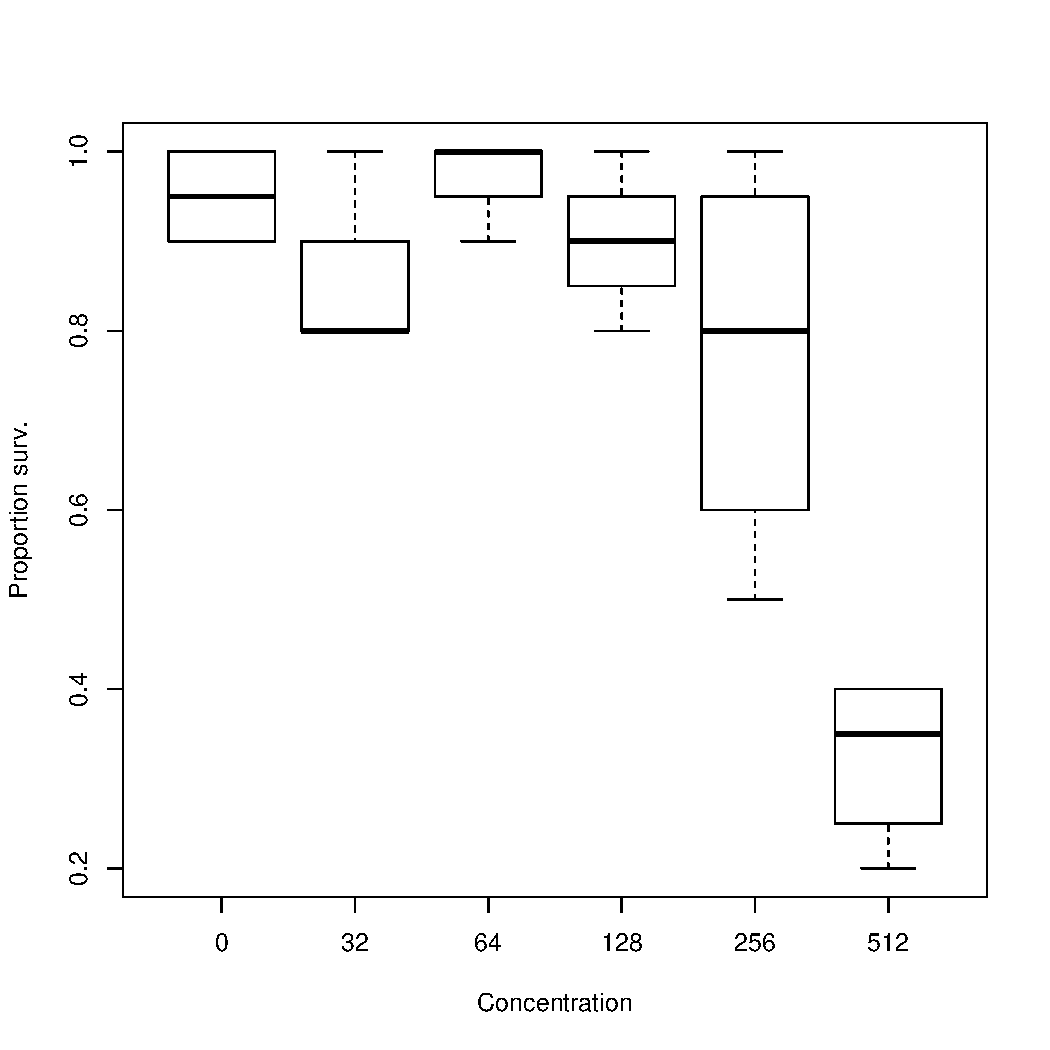
\includegraphics[width=0.5\textwidth]{figure/bin_raw_plot} 

\end{knitrout}


\subsubsection{Transforming data}
Next we arcsin transform the proportions:
\begin{knitrout}
\definecolor{shadecolor}{rgb}{0.969, 0.969, 0.969}\color{fgcolor}\begin{kframe}
\begin{alltt}
\hlstd{dfm}\hlopt{$}\hlstd{y_asin} \hlkwb{<-} \hlkwd{ifelse}\hlstd{(dfm}\hlopt{$}\hlstd{y} \hlopt{==} \hlnum{1}\hlstd{,} \hlkwd{asin}\hlstd{(}\hlnum{1}\hlstd{)} \hlopt{-} \hlkwd{asin}\hlstd{(}\hlkwd{sqrt}\hlstd{(}\hlnum{1}\hlopt{/}\hlnum{40}\hlstd{)),}
                                        \hlkwd{ifelse}\hlstd{(dfm}\hlopt{$}\hlstd{y} \hlopt{==} \hlnum{0}\hlstd{,} \hlkwd{asin}\hlstd{(}\hlkwd{sqrt}\hlstd{(}\hlnum{1}\hlopt{/}\hlnum{40}\hlstd{)),}
                                                \hlkwd{asin}\hlstd{(}\hlkwd{sqrt}\hlstd{(dfm}\hlopt{$}\hlstd{y))}
                                                \hlstd{)}
                                        \hlstd{)}
\end{alltt}
\end{kframe}
\end{knitrout}


\begin{knitrout}
\definecolor{shadecolor}{rgb}{0.969, 0.969, 0.969}\color{fgcolor}\begin{kframe}
\begin{alltt}
\hlkwd{boxplot}\hlstd{(y_asin} \hlopt{~} \hlstd{conc,} \hlkwc{data} \hlstd{= dfm,}
        \hlkwc{xlab} \hlstd{=} \hlstr{'Concentration'}\hlstd{,} \hlkwc{ylab} \hlstd{=} \hlstr{'Proportion surv.'}\hlstd{)}
\end{alltt}
\end{kframe}
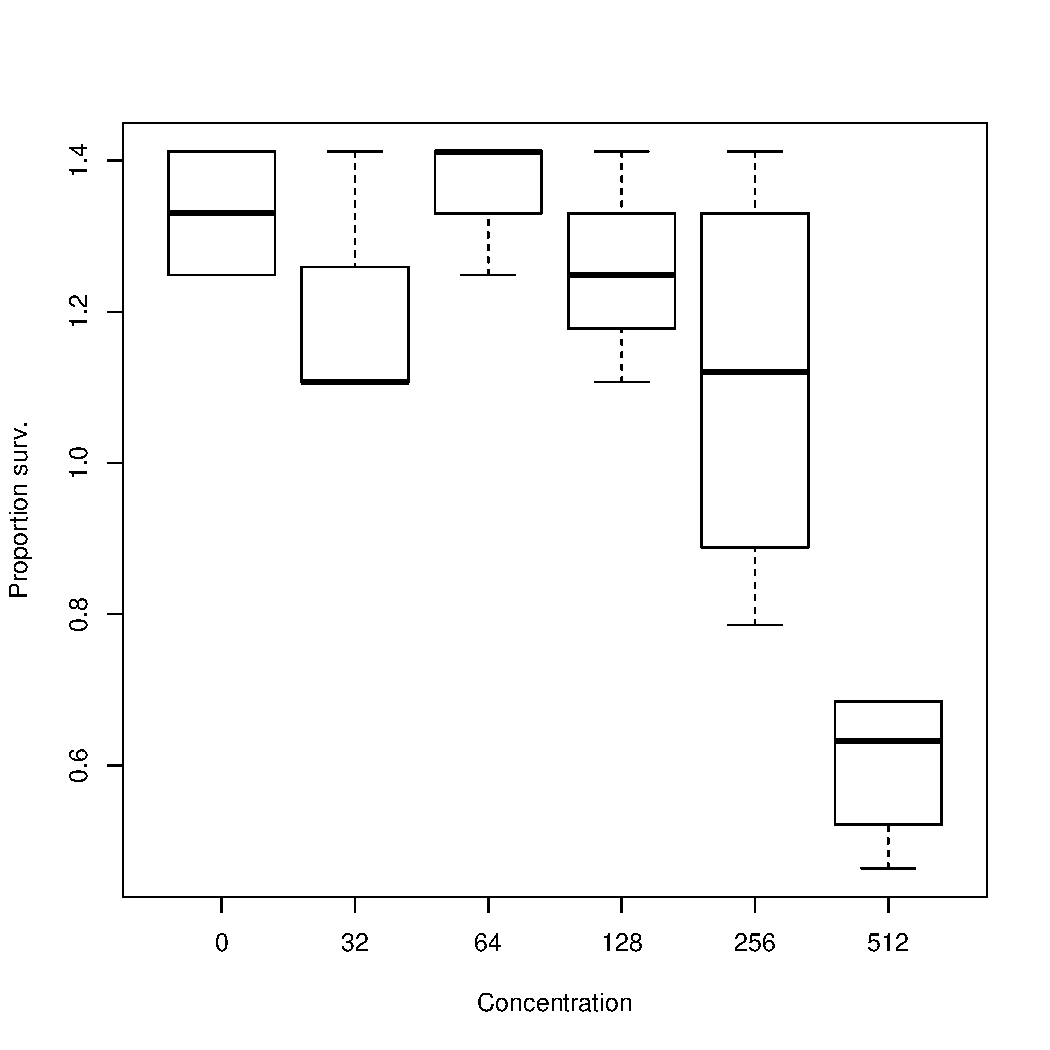
\includegraphics[width=0.5\textwidth]{figure/bin_trans_plot} 

\end{knitrout}

\subsubsection{Analysing data}
We will use the bbmle-package \citation{bolker_bbmle:_2014} to fit the models, as we used this also for the simulations.
However, also standard R functions can be use (see below).
Let's start with the model assuming a normal distribution of transformed proportions.

\begin{knitrout}
\definecolor{shadecolor}{rgb}{0.969, 0.969, 0.969}\color{fgcolor}\begin{kframe}
\begin{alltt}
\hlkwd{require}\hlstd{(bbmle)}
\hlstd{mod_normal} \hlkwb{<-} \hlkwd{mle2}\hlstd{(y_asin} \hlopt{~} \hlkwd{dnorm}\hlstd{(}\hlkwc{mean} \hlstd{= mu,} \hlkwc{sd} \hlstd{= s),}
                   \hlkwc{parameters} \hlstd{=} \hlkwd{list}\hlstd{(mu} \hlopt{~} \hlstd{conc, s} \hlopt{~} \hlnum{1}\hlstd{),}
                   \hlkwc{data} \hlstd{= dfm,}
                   \hlkwc{start} \hlstd{=} \hlkwd{list}\hlstd{(}\hlkwc{mu} \hlstd{=} \hlnum{0.5}\hlstd{,} \hlkwc{s} \hlstd{=} \hlnum{1}\hlstd{)}
                   \hlstd{)}
\hlkwd{summary}\hlstd{(mod_normal)}
\end{alltt}
\begin{verbatim}
## Maximum likelihood estimation
## 
## Call:
## mle2(minuslogl = y_asin ~ dnorm(mean = mu, sd = s), start = list(mu = 0.5, 
##     s = 1), data = dfm, parameters = list(mu ~ conc, s ~ 1))
## 
## Coefficients:
##                Estimate Std. Error z value   Pr(z)    
## mu.(Intercept)   1.3305     0.0666   19.97 < 2e-16 ***
## mu.conc32       -0.1472     0.0942   -1.56   0.118    
## mu.conc64        0.0407     0.0942    0.43   0.665    
## mu.conc128      -0.0762     0.0942   -0.81   0.419    
## mu.conc256      -0.2211     0.0942   -2.35   0.019 *  
## mu.conc512      -0.7274     0.0942   -7.72 1.2e-14 ***
## s                0.1333     0.0192    6.93 4.3e-12 ***
## ---
## Signif. codes:  0 '***' 0.001 '**' 0.01 '*' 0.05 '.' 0.1 ' ' 1
## 
## -2 log L: -28.64
\end{verbatim}
\end{kframe}
\end{knitrout}
This may gives some warnings as we did not put boundaries on the parameters (s cannot be 0 or lower), however we can ignore them.
The summary gives us the estimated parameters, their standard error and accompanying p-values.
Note that this model is parametrised a contrast to the control group so we can directly use the summary-output to determine the LOEC.
Note that these p-values are not adjusted for multiple testing (you can use p.adjust() for this).

The perform a Likelihood-Ratio-Test we specify a null model and compare both.
\begin{knitrout}
\definecolor{shadecolor}{rgb}{0.969, 0.969, 0.969}\color{fgcolor}\begin{kframe}
\begin{alltt}
\hlstd{mod_normal.null} \hlkwb{<-} \hlkwd{update}\hlstd{(mod_normal,}
                     \hlkwc{parameters} \hlstd{=} \hlkwd{list}\hlstd{(mu} \hlopt{~} \hlnum{1}\hlstd{, sd} \hlopt{~} \hlnum{1}\hlstd{)}
                     \hlstd{)}
\hlkwd{anova}\hlstd{(mod_normal, mod_normal.null)}
\end{alltt}
\begin{verbatim}
## Likelihood Ratio Tests
## Model 1: mod_normal, y_asin~dnorm(mean=mu,sd=s): mu~conc, s~1
## Model 2: mod_normal.null, y_asin~dnorm(mean=mu,sd=s): mu~1, sd~1
##   Tot Df Deviance Chisq Df Pr(>Chisq)    
## 1      7   -28.64                        
## 2      2     8.49  37.1  5    5.7e-07 ***
## ---
## Signif. codes:  0 '***' 0.001 '**' 0.01 '*' 0.05 '.' 0.1 ' ' 1
\end{verbatim}
\end{kframe}
\end{knitrout}

With base R we could do:
\begin{knitrout}
\definecolor{shadecolor}{rgb}{0.969, 0.969, 0.969}\color{fgcolor}\begin{kframe}
\begin{alltt}
\hlstd{mod_normal} \hlkwb{<-} \hlkwd{lm}\hlstd{(y_asin} \hlopt{~} \hlstd{conc,} \hlkwc{data} \hlstd{= dfm)}
\hlkwd{drop1}\hlstd{(mod_normal,} \hlkwc{test} \hlstd{=} \hlstr{'Chisq'}\hlstd{)}
\end{alltt}
\begin{verbatim}
## Single term deletions
## 
## Model:
## y_asin ~ conc
##        Df Sum of Sq   RSS   AIC Pr(>Chi)    
## <none>              0.426 -84.7             
## conc    5      1.57 2.001 -57.6  5.7e-07 ***
## ---
## Signif. codes:  0 '***' 0.001 '**' 0.01 '*' 0.05 '.' 0.1 ' ' 1
\end{verbatim}
\end{kframe}
\end{knitrout}
or using the lmtest package \citep{zeileis_diagnostic_2002}:
\begin{knitrout}
\definecolor{shadecolor}{rgb}{0.969, 0.969, 0.969}\color{fgcolor}\begin{kframe}
\begin{alltt}
\hlkwd{require}\hlstd{(lmtest)}
\hlkwd{lrtest}\hlstd{(mod_normal)}
\end{alltt}
\begin{verbatim}
## Likelihood ratio test
## 
## Model 1: y_asin ~ conc
## Model 2: y_asin ~ 1
##   #Df LogLik Df Chisq Pr(>Chisq)    
## 1   7  14.32                        
## 2   2  -4.24 -5  37.1    5.7e-07 ***
## ---
## Signif. codes:  0 '***' 0.001 '**' 0.01 '*' 0.05 '.' 0.1 ' ' 1
\end{verbatim}
\end{kframe}
\end{knitrout}



Next we assume that the number of surviving larvals are drawn from a binomial distribution.
First we backtransform the proportions reported to counts of surviving and dead larvals:
\begin{knitrout}
\definecolor{shadecolor}{rgb}{0.969, 0.969, 0.969}\color{fgcolor}\begin{kframe}
\begin{alltt}
\hlstd{dfm}\hlopt{$}\hlstd{surv} \hlkwb{<-} \hlstd{dfm}\hlopt{$}\hlstd{y} \hlopt{*} \hlnum{10}
\hlstd{dfm}\hlopt{$}\hlstd{dead} \hlkwb{<-} \hlnum{10} \hlopt{-} \hlstd{dfm}\hlopt{$}\hlstd{surv}
\end{alltt}
\end{kframe}
\end{knitrout}

And then we specify the logistic model:
\begin{knitrout}
\definecolor{shadecolor}{rgb}{0.969, 0.969, 0.969}\color{fgcolor}\begin{kframe}
\begin{alltt}
\hlstd{mod_bin} \hlkwb{<-} \hlkwd{mle2}\hlstd{(surv} \hlopt{~} \hlkwd{dbinom}\hlstd{(}\hlkwc{size} \hlstd{=} \hlnum{10}\hlstd{,} \hlkwc{prob} \hlstd{=} \hlkwd{plogis}\hlstd{(lp)),}
                \hlkwc{parameters} \hlstd{=} \hlkwd{list}\hlstd{(lp} \hlopt{~} \hlstd{conc),}
                \hlkwc{data} \hlstd{= dfm,}
                \hlkwc{start} \hlstd{=} \hlkwd{list}\hlstd{(}\hlkwc{lp} \hlstd{=} \hlnum{0}\hlstd{)}
                \hlstd{)}
\hlkwd{summary}\hlstd{(mod_bin)}
\end{alltt}
\begin{verbatim}
## Maximum likelihood estimation
## 
## Call:
## mle2(minuslogl = surv ~ dbinom(size = 10, prob = plogis(lp)), 
##     start = list(lp = 0), data = dfm, parameters = list(lp ~ 
##         conc))
## 
## Coefficients:
##                Estimate Std. Error z value   Pr(z)    
## lp.(Intercept)    2.944      0.725    4.06 4.9e-05 ***
## lp.conc32        -1.210      0.850   -1.42   0.155    
## lp.conc64         0.719      1.246    0.58   0.564    
## lp.conc128       -0.747      0.897   -0.83   0.405    
## lp.conc256       -1.708      0.818   -2.09   0.037 *  
## lp.conc512       -3.675      0.800   -4.59 4.4e-06 ***
## ---
## Signif. codes:  0 '***' 0.001 '**' 0.01 '*' 0.05 '.' 0.1 ' ' 1
## 
## -2 log L: 60.86
\end{verbatim}
\end{kframe}
\end{knitrout}

And perform the LRT
\begin{knitrout}
\definecolor{shadecolor}{rgb}{0.969, 0.969, 0.969}\color{fgcolor}\begin{kframe}
\begin{alltt}
\hlstd{mod_bin.null} \hlkwb{<-} \hlkwd{update}\hlstd{(mod_bin,}
                       \hlkwc{parameters} \hlstd{=} \hlkwd{list}\hlstd{(lp} \hlopt{~} \hlnum{1}\hlstd{))}
\hlkwd{anova}\hlstd{(mod_bin, mod_bin.null)}
\end{alltt}
\begin{verbatim}
## Likelihood Ratio Tests
## Model 1: mod_bin, surv~dbinom(size=10,prob=plogis(lp)): lp~conc
## Model 2: mod_bin.null, surv~dbinom(size=10,prob=plogis(lp)): lp~1
##   Tot Df Deviance Chisq Df Pr(>Chisq)    
## 1      6     60.9                        
## 2      1    125.6  64.8  5    1.2e-12 ***
## ---
## Signif. codes:  0 '***' 0.001 '**' 0.01 '*' 0.05 '.' 0.1 ' ' 1
\end{verbatim}
\end{kframe}
\end{knitrout}


With base R we could use
\begin{knitrout}
\definecolor{shadecolor}{rgb}{0.969, 0.969, 0.969}\color{fgcolor}\begin{kframe}
\begin{alltt}
\hlstd{mod_bin_b} \hlkwb{<-} \hlkwd{glm}\hlstd{(}\hlkwd{cbind}\hlstd{(surv, dead)} \hlopt{~} \hlstd{conc,} \hlkwc{data} \hlstd{= dfm,} \hlkwc{family} \hlstd{=} \hlkwd{binomial}\hlstd{(}\hlkwc{link} \hlstd{=} \hlstr{'logit'}\hlstd{))}
\hlkwd{summary}\hlstd{(mod_bin_b)}
\end{alltt}
\begin{verbatim}
## 
## Call:
## glm(formula = cbind(surv, dead) ~ conc, family = binomial(link = "logit"), 
##     data = dfm)
## 
## Deviance Residuals: 
##    Min      1Q  Median      3Q     Max  
## -1.898  -0.572   0.000   0.787   2.258  
## 
## Coefficients:
##             Estimate Std. Error z value Pr(>|z|)    
## (Intercept)    2.944      0.725    4.06  4.9e-05 ***
## conc32        -1.210      0.850   -1.42    0.155    
## conc64         0.719      1.246    0.58    0.564    
## conc128       -0.747      0.897   -0.83    0.405    
## conc256       -1.708      0.818   -2.09    0.037 *  
## conc512       -3.675      0.800   -4.59  4.4e-06 ***
## ---
## Signif. codes:  0 '***' 0.001 '**' 0.01 '*' 0.05 '.' 0.1 ' ' 1
## 
## (Dispersion parameter for binomial family taken to be 1)
## 
##     Null deviance: 88.672  on 23  degrees of freedom
## Residual deviance: 23.889  on 18  degrees of freedom
## AIC: 72.86
## 
## Number of Fisher Scoring iterations: 5
\end{verbatim}
\begin{alltt}
\hlkwd{drop1}\hlstd{(mod_bin_b,} \hlkwc{test} \hlstd{=} \hlstr{'Chisq'}\hlstd{)}
\end{alltt}
\begin{verbatim}
## Single term deletions
## 
## Model:
## cbind(surv, dead) ~ conc
##        Df Deviance   AIC  LRT Pr(>Chi)    
## <none>        23.9  72.9                  
## conc    5     88.7 127.6 64.8  1.2e-12 ***
## ---
## Signif. codes:  0 '***' 0.001 '**' 0.01 '*' 0.05 '.' 0.1 ' ' 1
\end{verbatim}
\end{kframe}
\end{knitrout}



\subsection{Count data}
\subsubsection{Introduction}
In this example we will analyse data from \citep{brock_minimum_2014}.
The data are count of mayfly larvae in Macroinvertebrate Artificial Substrate Samplers in 18 mesocosms at one sampling day.
There are 5 Treatments and one control group.

First we load the data and bring it to the long format and remove NA values.
\begin{knitrout}
\definecolor{shadecolor}{rgb}{0.969, 0.969, 0.969}\color{fgcolor}\begin{kframe}
\begin{alltt}
\hlstd{df} \hlkwb{<-} \hlkwd{read.table}\hlstd{(}\hlkwc{header} \hlstd{=} \hlnum{TRUE}\hlstd{,} \hlkwc{text} \hlstd{=} \hlstr{'Control  T0.1	T0.3	T1	T3	T10
175	29	27	36	26	20
65	114	78	11	13	37
154	72	27	105	33	NA
83	NA	NA	NA	NA	NA
'}\hlstd{)}
\hlstd{dfm} \hlkwb{<-} \hlkwd{melt}\hlstd{(df,} \hlkwc{value.name} \hlstd{=} \hlstr{'n'}\hlstd{,} \hlkwc{variable.name} \hlstd{=} \hlstr{'treatment'}\hlstd{)}
\hlstd{dfm} \hlkwb{<-} \hlstd{dfm[}\hlopt{!}\hlkwd{is.na}\hlstd{(dfm[}\hlstr{'n'}\hlstd{]), ]}
\hlkwd{head}\hlstd{(dfm)}
\end{alltt}
\begin{verbatim}
##   treatment   n
## 1   Control 175
## 2   Control  65
## 3   Control 154
## 4   Control  83
## 5      T0.1  29
## 6      T0.1 114
\end{verbatim}
\end{kframe}
\end{knitrout}

	
Next we have a look at the data:
\begin{knitrout}
\definecolor{shadecolor}{rgb}{0.969, 0.969, 0.969}\color{fgcolor}\begin{kframe}
\begin{alltt}
\hlkwd{boxplot}\hlstd{(n} \hlopt{~} \hlstd{treatment,} \hlkwc{data} \hlstd{= dfm,} \hlkwc{xlab} \hlstd{=} \hlstr{'Treatment'}\hlstd{,} \hlkwc{ylab} \hlstd{=} \hlstr{'Count'}\hlstd{)}
\end{alltt}
\end{kframe}
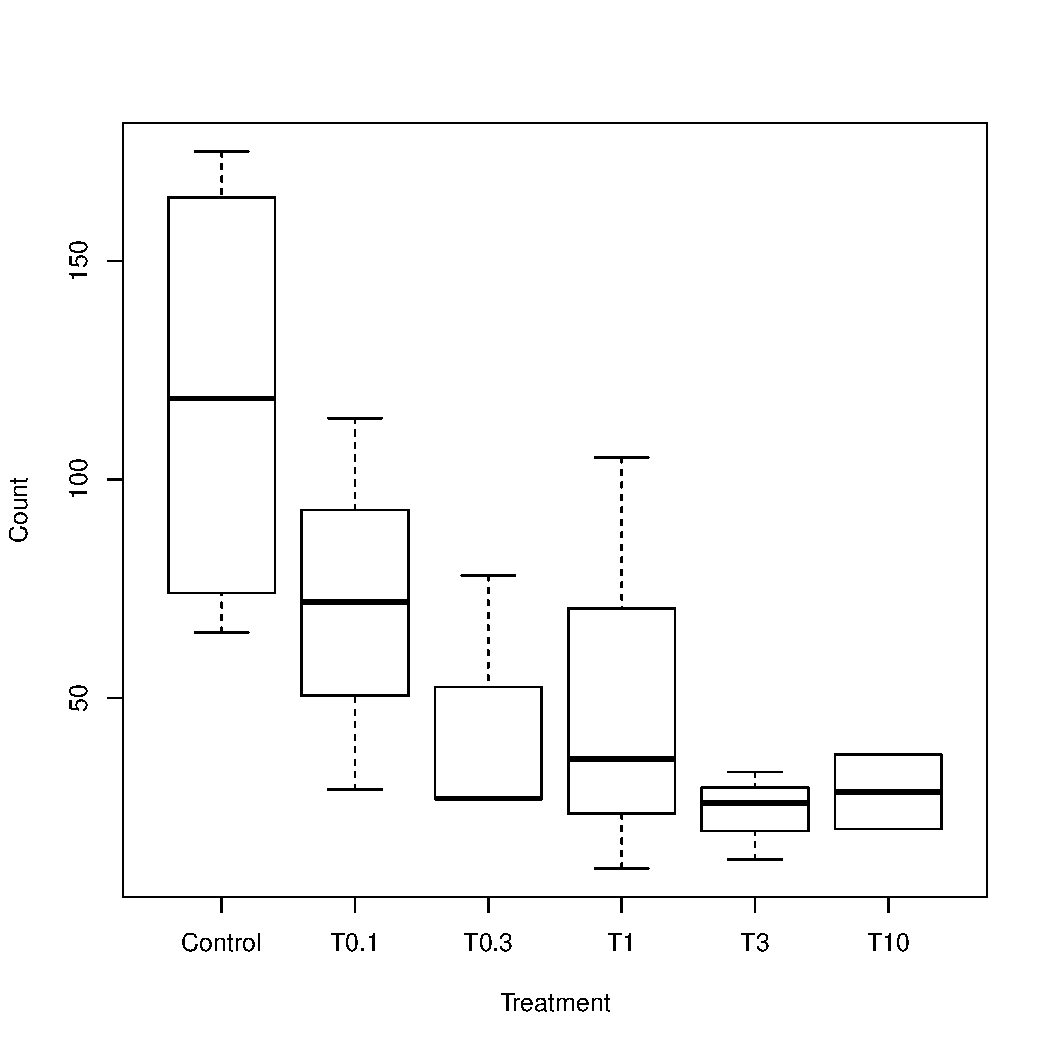
\includegraphics[width=0.5\textwidth]{figure/count_raw_plot} 

\end{knitrout}


\subsubsection{Transforming data}
Next we transform the data using a ln(Ax + 1) transformation:

\begin{knitrout}
\definecolor{shadecolor}{rgb}{0.969, 0.969, 0.969}\color{fgcolor}\begin{kframe}
\begin{alltt}
\hlstd{A} \hlkwb{<-} \hlnum{1} \hlopt{/} \hlkwd{min}\hlstd{(dfm}\hlopt{$}\hlstd{n[dfm}\hlopt{$}\hlstd{n} \hlopt{!=} \hlnum{0}\hlstd{])}
\hlstd{dfm}\hlopt{$}\hlstd{nt} \hlkwb{<-} \hlkwd{log}\hlstd{(A} \hlopt{*} \hlstd{dfm}\hlopt{$}\hlstd{n} \hlopt{+} \hlnum{1}\hlstd{)}
\end{alltt}
\end{kframe}
\end{knitrout}

\begin{knitrout}
\definecolor{shadecolor}{rgb}{0.969, 0.969, 0.969}\color{fgcolor}\begin{kframe}
\begin{alltt}
\hlkwd{boxplot}\hlstd{(nt} \hlopt{~} \hlstd{treatment,} \hlkwc{data} \hlstd{= dfm,}
        \hlkwc{xlab} \hlstd{=} \hlstr{'Treatment'}\hlstd{,} \hlkwc{ylab} \hlstd{=} \hlstr{'Transf. Counts'}\hlstd{)}
\end{alltt}
\end{kframe}
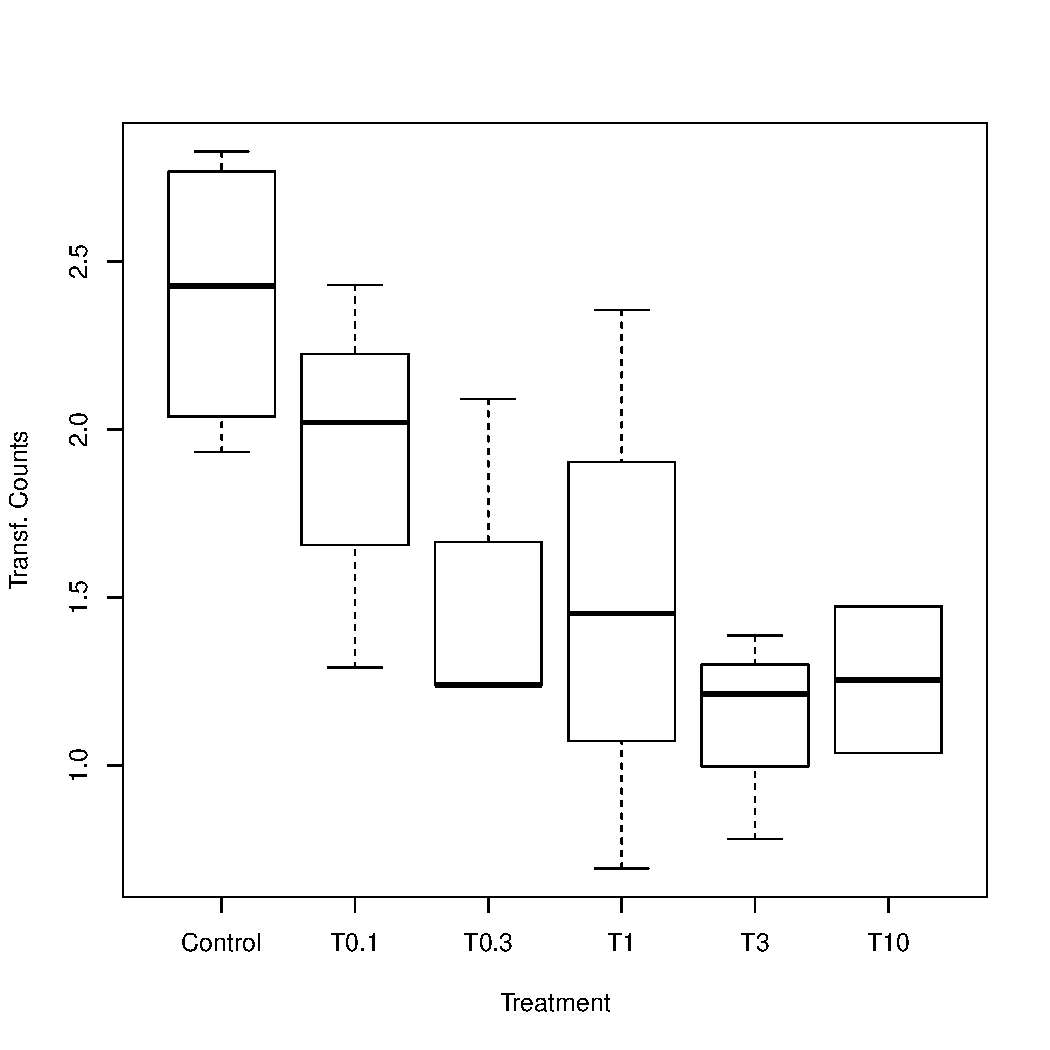
\includegraphics[width=0.5\textwidth]{figure/plot_count_trans} 

\end{knitrout}


\subsection{Analsying data}
Again we start with the model assuming a normal distribution of transformed counts:
\begin{knitrout}
\definecolor{shadecolor}{rgb}{0.969, 0.969, 0.969}\color{fgcolor}\begin{kframe}
\begin{alltt}
\hlstd{mod_normal} \hlkwb{<-} \hlkwd{mle2}\hlstd{(nt} \hlopt{~} \hlkwd{dnorm}\hlstd{(}\hlkwc{mean} \hlstd{= mu,} \hlkwc{sd} \hlstd{= s),}
                   \hlkwc{parameters} \hlstd{=} \hlkwd{list}\hlstd{(mu} \hlopt{~} \hlstd{treatment, s} \hlopt{~} \hlnum{1}\hlstd{),}
                   \hlkwc{data} \hlstd{= dfm,}
                   \hlkwc{start} \hlstd{=} \hlkwd{list}\hlstd{(}\hlkwc{mu} \hlstd{=} \hlkwd{mean}\hlstd{(dfm}\hlopt{$}\hlstd{nt),} \hlkwc{s} \hlstd{=} \hlkwd{sd}\hlstd{(dfm}\hlopt{$}\hlstd{nt)))}
\hlkwd{summary}\hlstd{(mod_normal)}
\end{alltt}
\begin{verbatim}
## Maximum likelihood estimation
## 
## Call:
## mle2(minuslogl = nt ~ dnorm(mean = mu, sd = s), start = list(mu = mean(dfm$nt), 
##     s = sd(dfm$nt)), data = dfm, parameters = list(mu ~ treatment, 
##     s ~ 1))
## 
## Coefficients:
##                  Estimate Std. Error z value   Pr(z)    
## mu.(Intercept)     2.4035     0.2169   11.08 < 2e-16 ***
## mu.treatmentT0.1  -0.4894     0.3313   -1.48 0.13956    
## mu.treatmentT0.3  -0.8801     0.3313   -2.66 0.00789 ** 
## mu.treatmentT1    -0.9032     0.3313   -2.73 0.00640 ** 
## mu.treatmentT3    -1.2771     0.3313   -3.86 0.00012 ***
## mu.treatmentT10   -1.1488     0.3756   -3.06 0.00222 ** 
## s                  0.4337     0.0723    6.00   2e-09 ***
## ---
## Signif. codes:  0 '***' 0.001 '**' 0.01 '*' 0.05 '.' 0.1 ' ' 1
## 
## -2 log L: 21.01
\end{verbatim}
\begin{alltt}
\hlstd{mod_normal.null} \hlkwb{<-} \hlkwd{update}\hlstd{(mod_normal,}
                          \hlkwc{parameters} \hlstd{=} \hlkwd{list}\hlstd{(mu} \hlopt{~} \hlnum{1}\hlstd{, s} \hlopt{~} \hlnum{1}\hlstd{))}
\hlkwd{anova}\hlstd{(mod_normal, mod_normal.null)}
\end{alltt}
\begin{verbatim}
## Likelihood Ratio Tests
## Model 1: mod_normal, nt~dnorm(mean=mu,sd=s): mu~treatment, s~1
## Model 2: mod_normal.null, nt~dnorm(mean=mu,sd=s): mu~1, s~1
##   Tot Df Deviance Chisq Df Pr(>Chisq)  
## 1      7     21.0                      
## 2      2     34.3  13.3  5      0.021 *
## ---
## Signif. codes:  0 '***' 0.001 '**' 0.01 '*' 0.05 '.' 0.1 ' ' 1
\end{verbatim}
\end{kframe}
\end{knitrout}

With base R you could do:
\begin{knitrout}
\definecolor{shadecolor}{rgb}{0.969, 0.969, 0.969}\color{fgcolor}\begin{kframe}
\begin{alltt}
\hlstd{mod_normal_b} \hlkwb{<-} \hlkwd{lm}\hlstd{(nt} \hlopt{~} \hlstd{treatment,} \hlkwc{data} \hlstd{= dfm)}
\hlkwd{summary}\hlstd{(mod_normal_b)}
\hlkwd{drop1}\hlstd{(mod_normal_b,} \hlkwc{test} \hlstd{=} \hlstr{'Chisq'}\hlstd{)}
\end{alltt}
\end{kframe}
\end{knitrout}


Next we analyse the raw counts assuming a poisson distribution with a log link:
\begin{knitrout}
\definecolor{shadecolor}{rgb}{0.969, 0.969, 0.969}\color{fgcolor}\begin{kframe}
\begin{alltt}
\hlstd{mod_pois} \hlkwb{<-} \hlkwd{mle2}\hlstd{(n} \hlopt{~} \hlkwd{dpois}\hlstd{(}\hlkwc{lambda} \hlstd{=} \hlkwd{exp}\hlstd{(logmu)),}
                   \hlkwc{parameters} \hlstd{=} \hlkwd{list}\hlstd{(logmu} \hlopt{~} \hlstd{treatment),}
                   \hlkwc{data} \hlstd{= dfm,}
                   \hlkwc{start} \hlstd{=} \hlkwd{list}\hlstd{(}\hlkwc{logmu} \hlstd{=} \hlkwd{mean}\hlstd{(dfm}\hlopt{$}\hlstd{nt)))}
\hlkwd{summary}\hlstd{(mod_pois)}
\end{alltt}
\begin{verbatim}
## Maximum likelihood estimation
## 
## Call:
## mle2(minuslogl = n ~ dpois(lambda = exp(logmu)), start = list(logmu = mean(dfm$nt)), 
##     data = dfm, parameters = list(logmu ~ treatment))
## 
## Coefficients:
##                     Estimate Std. Error z value   Pr(z)    
## logmu.(Intercept)     4.7812     0.0458  104.42 < 2e-16 ***
## logmu.treatmentT0.1  -0.5093     0.0821   -6.20 5.7e-10 ***
## logmu.treatmentT0.3  -0.9970     0.0983  -10.14 < 2e-16 ***
## logmu.treatmentT1    -0.8560     0.0931   -9.19 < 2e-16 ***
## logmu.treatmentT3    -1.6032     0.1264  -12.68 < 2e-16 ***
## logmu.treatmentT10   -1.4313     0.1401  -10.21 < 2e-16 ***
## ---
## Signif. codes:  0 '***' 0.001 '**' 0.01 '*' 0.05 '.' 0.1 ' ' 1
## 
## -2 log L: 375.6
\end{verbatim}
\end{kframe}
\end{knitrout}

Or with base R
\begin{knitrout}
\definecolor{shadecolor}{rgb}{0.969, 0.969, 0.969}\color{fgcolor}\begin{kframe}
\begin{alltt}
\hlstd{mod_pois} \hlkwb{<-} \hlkwd{glm}\hlstd{(n} \hlopt{~} \hlstd{treatment,} \hlkwc{data} \hlstd{= dfm,} \hlkwc{family} \hlstd{=} \hlkwd{poisson}\hlstd{(}\hlkwc{link} \hlstd{=} \hlstr{'log'}\hlstd{))}
\hlkwd{summary}\hlstd{(mod_pois)}
\end{alltt}
\end{kframe}
\end{knitrout}

But is a poisson distribution appropriate here? 
A property of the poisson distribution is that its variance is equal to the mean. A simple diagnostic would be to plot group variances vs group means, other more formal statistics are also available.


\begin{knitrout}
\definecolor{shadecolor}{rgb}{0.969, 0.969, 0.969}\color{fgcolor}\begin{kframe}
\begin{alltt}
\hlkwd{require}\hlstd{(plyr)}
\hlstd{musd} \hlkwb{<-} \hlkwd{ddply}\hlstd{(dfm,} \hlkwd{.}\hlstd{(treatment), summarise,}
              \hlkwc{mu} \hlstd{=} \hlkwd{mean}\hlstd{(n),}
              \hlkwc{var} \hlstd{=} \hlkwd{var}\hlstd{(n))}
\hlstd{musd}
\end{alltt}
\begin{verbatim}
##   treatment     mu    var
## 1   Control 119.25 2857.6
## 2      T0.1  71.67 1806.3
## 3      T0.3  44.00  867.0
## 4        T1  50.67 2370.3
## 5        T3  24.00  103.0
## 6       T10  28.50  144.5
\end{verbatim}
\begin{alltt}
\hlkwd{plot}\hlstd{(var} \hlopt{~} \hlstd{mu,} \hlkwc{data} \hlstd{= musd,} \hlkwc{xlab} \hlstd{=} \hlstr{'mean'}\hlstd{,} \hlkwc{ylab} \hlstd{=} \hlstr{'Variance'}\hlstd{)}
\hlkwd{abline}\hlstd{(}\hlkwc{a} \hlstd{=} \hlnum{0}\hlstd{,} \hlkwc{b} \hlstd{=} \hlnum{1}\hlstd{,} \hlkwc{col} \hlstd{=} \hlstr{'darkblue'}\hlstd{,} \hlkwc{lwd} \hlstd{=} \hlnum{2}\hlstd{)}
\hlkwd{curve}\hlstd{(x} \hlopt{+} \hlstd{(x}\hlopt{^}\hlnum{2} \hlopt{/} \hlnum{3.91}\hlstd{),} \hlkwc{from} \hlstd{=} \hlnum{24}\hlstd{,} \hlkwc{to} \hlstd{=} \hlnum{119.25}\hlstd{,} \hlkwc{add} \hlstd{=} \hlnum{TRUE}\hlstd{,} \hlkwc{col} \hlstd{=} \hlstr{'darkred'}\hlstd{,} \hlkwc{lwd} \hlstd{=} \hlnum{2}\hlstd{)}
\hlkwd{legend}\hlstd{(}\hlstr{'topleft'}\hlstd{,} \hlkwd{c}\hlstd{(}\hlstr{'NB(k = 3.91)'}\hlstd{,} \hlstr{'Poisson'}\hlstd{),}
       \hlkwc{col} \hlstd{=} \hlkwd{c}\hlstd{(}\hlstr{'darkred'}\hlstd{,} \hlstr{'darkblue'}\hlstd{),}
       \hlkwc{lty} \hlstd{=} \hlkwd{c}\hlstd{(}\hlnum{1}\hlstd{,}\hlnum{1}\hlstd{),}
       \hlkwc{lwd} \hlstd{=} \hlkwd{c}\hlstd{(}\hlnum{2}\hlstd{,}\hlnum{2}\hlstd{))}
\end{alltt}
\end{kframe}
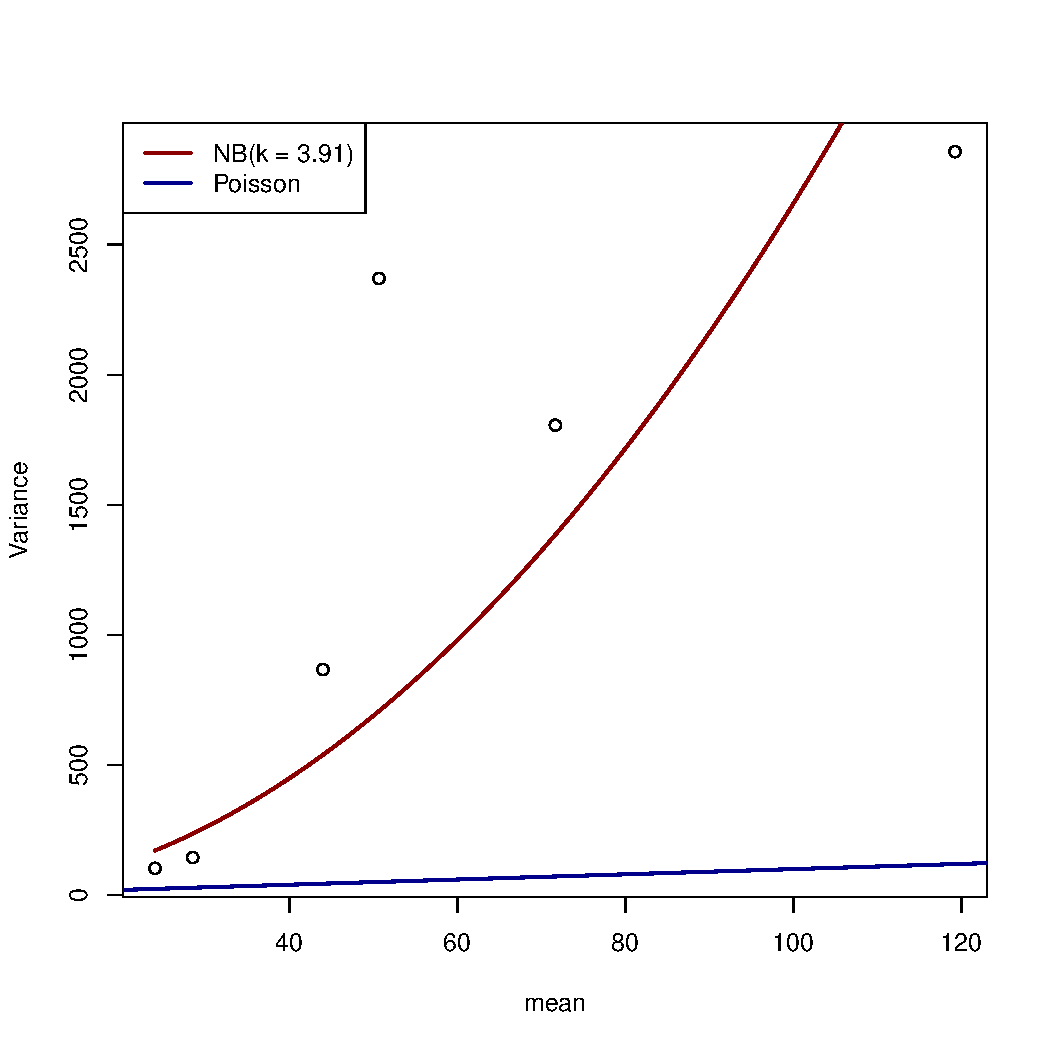
\includegraphics[width=0.5\textwidth]{figure/mod_count_meanvar} 

\end{knitrout}

We clearly see that the variance increases much more than would be expected under the poisson distribution (the data is overdispersed).
One possibility to deal with overdispersion is using a negative binomial distribution:

\begin{knitrout}
\definecolor{shadecolor}{rgb}{0.969, 0.969, 0.969}\color{fgcolor}\begin{kframe}
\begin{alltt}
\hlstd{mod_negbin} \hlkwb{<-} \hlkwd{mle2}\hlstd{(n} \hlopt{~} \hlkwd{dnbinom}\hlstd{(}\hlkwc{mu} \hlstd{=} \hlkwd{exp}\hlstd{(logmu),} \hlkwc{size} \hlstd{= k),}
                   \hlkwc{parameters} \hlstd{=} \hlkwd{list}\hlstd{(logmu} \hlopt{~} \hlstd{treatment, k} \hlopt{~} \hlnum{1}\hlstd{),}
                   \hlkwc{data} \hlstd{= dfm,}
                   \hlkwc{start} \hlstd{=} \hlkwd{list}\hlstd{(}\hlkwc{logmu} \hlstd{=} \hlkwd{log}\hlstd{(}\hlkwd{mean}\hlstd{(dfm}\hlopt{$}\hlstd{n)),} \hlkwc{k} \hlstd{=} \hlnum{1}\hlstd{))}
\hlkwd{summary}\hlstd{(mod_negbin)}
\end{alltt}
\begin{verbatim}
## Maximum likelihood estimation
## 
## Call:
## mle2(minuslogl = n ~ dnbinom(mu = exp(logmu), size = k), start = list(logmu = log(mean(dfm$n)), 
##     k = 1), data = dfm, parameters = list(logmu ~ treatment, 
##     k ~ 1))
## 
## Coefficients:
##                     Estimate Std. Error z value   Pr(z)    
## logmu.(Intercept)      4.781      0.257   18.60 < 2e-16 ***
## logmu.treatmentT0.1   -0.509      0.395   -1.29  0.1974    
## logmu.treatmentT0.3   -0.997      0.399   -2.50  0.0124 *  
## logmu.treatmentT1     -0.856      0.398   -2.15  0.0313 *  
## logmu.treatmentT3     -1.603      0.407   -3.94 8.1e-05 ***
## logmu.treatmentT10    -1.431      0.460   -3.11  0.0019 ** 
## k                      3.906      1.366    2.86  0.0042 ** 
## ---
## Signif. codes:  0 '***' 0.001 '**' 0.01 '*' 0.05 '.' 0.1 ' ' 1
## 
## -2 log L: 167.2
\end{verbatim}
\begin{alltt}
\hlstd{mod_negbin.null} \hlkwb{<-} \hlkwd{update}\hlstd{(mod_negbin,}
                          \hlkwc{parameters} \hlstd{=} \hlkwd{list}\hlstd{(logmu} \hlopt{~} \hlnum{1}\hlstd{))}
\hlkwd{anova}\hlstd{(mod_negbin, mod_negbin.null)}
\end{alltt}
\begin{verbatim}
## Likelihood Ratio Tests
## Model 1: mod_negbin, n~dnbinom(mu=exp(logmu),size=k): logmu~treatment, k~1
## Model 2: mod_negbin.null, n~dnbinom(mu=exp(logmu),size=k): logmu~1
##   Tot Df Deviance Chisq Df Pr(>Chisq)  
## 1      7      167                      
## 2      2      181    14  5      0.016 *
## ---
## Signif. codes:  0 '***' 0.001 '**' 0.01 '*' 0.05 '.' 0.1 ' ' 1
\end{verbatim}
\end{kframe}
\end{knitrout}

Or using the MASS package \citep{venables_modern_2002}:
\begin{knitrout}
\definecolor{shadecolor}{rgb}{0.969, 0.969, 0.969}\color{fgcolor}\begin{kframe}
\begin{alltt}
\hlkwd{require}\hlstd{(MASS)}
\hlstd{mod_negbin_m} \hlkwb{<-} \hlkwd{glm.nb}\hlstd{(n} \hlopt{~} \hlstd{treatment,} \hlkwc{data} \hlstd{= dfm)}
\hlkwd{summary}\hlstd{(mod_negbin_m)}
\end{alltt}
\begin{verbatim}
## 
## Call:
## glm.nb(formula = n ~ treatment, data = dfm, init.theta = 3.905898474, 
##     link = log)
## 
## Deviance Residuals: 
##    Min      1Q  Median      3Q     Max  
## -2.255  -0.849  -0.302   0.595   1.590  
## 
## Coefficients:
##               Estimate Std. Error z value Pr(>|z|)    
## (Intercept)      4.781      0.257   18.60  < 2e-16 ***
## treatmentT0.1   -0.509      0.395   -1.29   0.1975    
## treatmentT0.3   -0.997      0.399   -2.50   0.0124 *  
## treatmentT1     -0.856      0.398   -2.15   0.0313 *  
## treatmentT3     -1.603      0.407   -3.94  8.1e-05 ***
## treatmentT10    -1.431      0.460   -3.11   0.0019 ** 
## ---
## Signif. codes:  0 '***' 0.001 '**' 0.01 '*' 0.05 '.' 0.1 ' ' 1
## 
## (Dispersion parameter for Negative Binomial(3.906) family taken to be 1)
## 
##     Null deviance: 39.057  on 17  degrees of freedom
## Residual deviance: 18.611  on 12  degrees of freedom
## AIC: 181.2
## 
## Number of Fisher Scoring iterations: 1
## 
## 
##               Theta:  3.91 
##           Std. Err.:  1.37 
## 
##  2 x log-likelihood:  -167.24
\end{verbatim}
\begin{alltt}
\hlkwd{lrtest}\hlstd{(mod_negbin_m)}
\end{alltt}
\begin{verbatim}
## Likelihood ratio test
## 
## Model 1: n ~ treatment
## Model 2: n ~ 1
##   #Df LogLik Df Chisq Pr(>Chisq)  
## 1   7  -83.6                      
## 2   2  -90.6 -5    14      0.016 *
## ---
## Signif. codes:  0 '***' 0.001 '**' 0.01 '*' 0.05 '.' 0.1 ' ' 1
\end{verbatim}
\end{kframe}
\end{knitrout}
Note, that we cannot use drop1() with glm.nb()!



\bibliography{references}
\bibliographystyle{apalike}


\end{document} 
